\chapter{Games}
\label{chap:games}
\todo{can extend both by including historical info}
In this chapter, the board games, Mastermind and Battleship, used for the experiments in chapter \ref{chap:experiments} will be introduced. The objective, rules and gameplay will be discussed. \todo{maybe explain why these two games were chosen? and/or why strategic board games?}

\section{Mastermind}
\label{sec:mastermind}

Mastermind is a 2-player board game. Both players have different tasks and roles, namely codebreaker and codemaker. Like the names imply, the task of one player is to make a code and the task of the other player is to break it. In this game, the codemaker generates the code from a pool of various coloured pins. The order of the colours matter. The game is usually played on a 10 x 4 board and 6 colours. The codemaker has an additional hidden row to hide his code. In each column, there is a hole for the codebreaker to put in a pin for his guess attempt. Additionally, in each row there are four smaller holes, which the codemaker uses to give feedback. The codemaker will use black/red to indicate colour and position are correct, white for correct colour, but wrong position, or leave it empty, if the colour is not available in the code \cite{Howtopla33:online}. A modern variation of the game board can be seen in figure \ref{fig:mastermind_board}.

\begin{figure}[H]
  \centering
  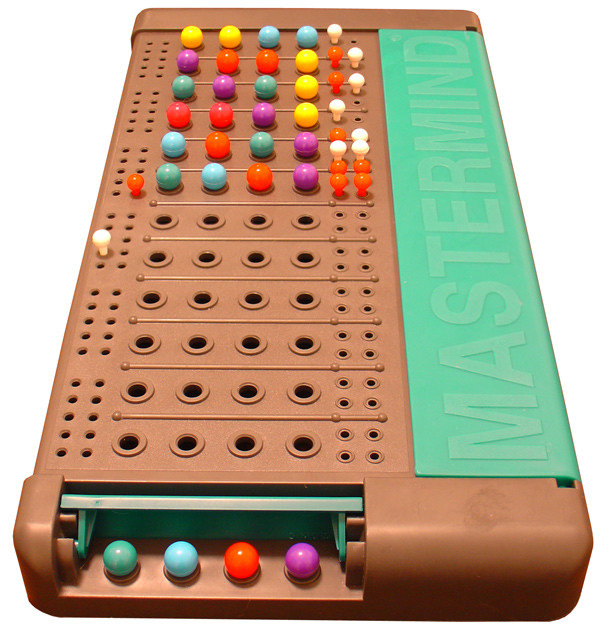
\includegraphics[scale=.25]{images/mastermind_board}
  \caption[Mastermind game board]{Mastermind game board with 12 rows and 6 colours. Additionally, a hidden row for the code, at the bottom. Source: Reprinted from \cite{enwiki:1122862799}}
  \label{fig:mastermind_board}
\end{figure}  

For the experiments, a game board of size 10 x 4 and 6 colours were used. \todo{verify}

\section{Battleship}
\label{ssec:battleship}
Battleship is another classic 2-player board game. The objective is to sink all enemy battleships. At the start of a game, each player has a pool of battleships with mixed lengths and has to place them, either horizontally, or vertically, on their own 10 x 10 board. The boards are kept hidden from each other. Typically, the length of the battleships ranges from two to five. 
%and the number of ships available for placement, decreases with increasing length, i.e. 5 x 2-size, 4 x 3-size, 3 x 4-size and 2 x 5-size battleships. 
These numbers were also used in the experiments \todo{verify. gehört das überhaupt hier rein? kann man doppelt machen, aber vllt hat das hier nichts zu suchen}. Ships are allowed to touch, but not to overlap. Alternately, players call out which coordinate they want to attack. The opponent responds with either \textit{hit}, or \textit{miss}, when the attacker hit a battleship, or not, respectively.

\begin{figure}[H]
  \centering
  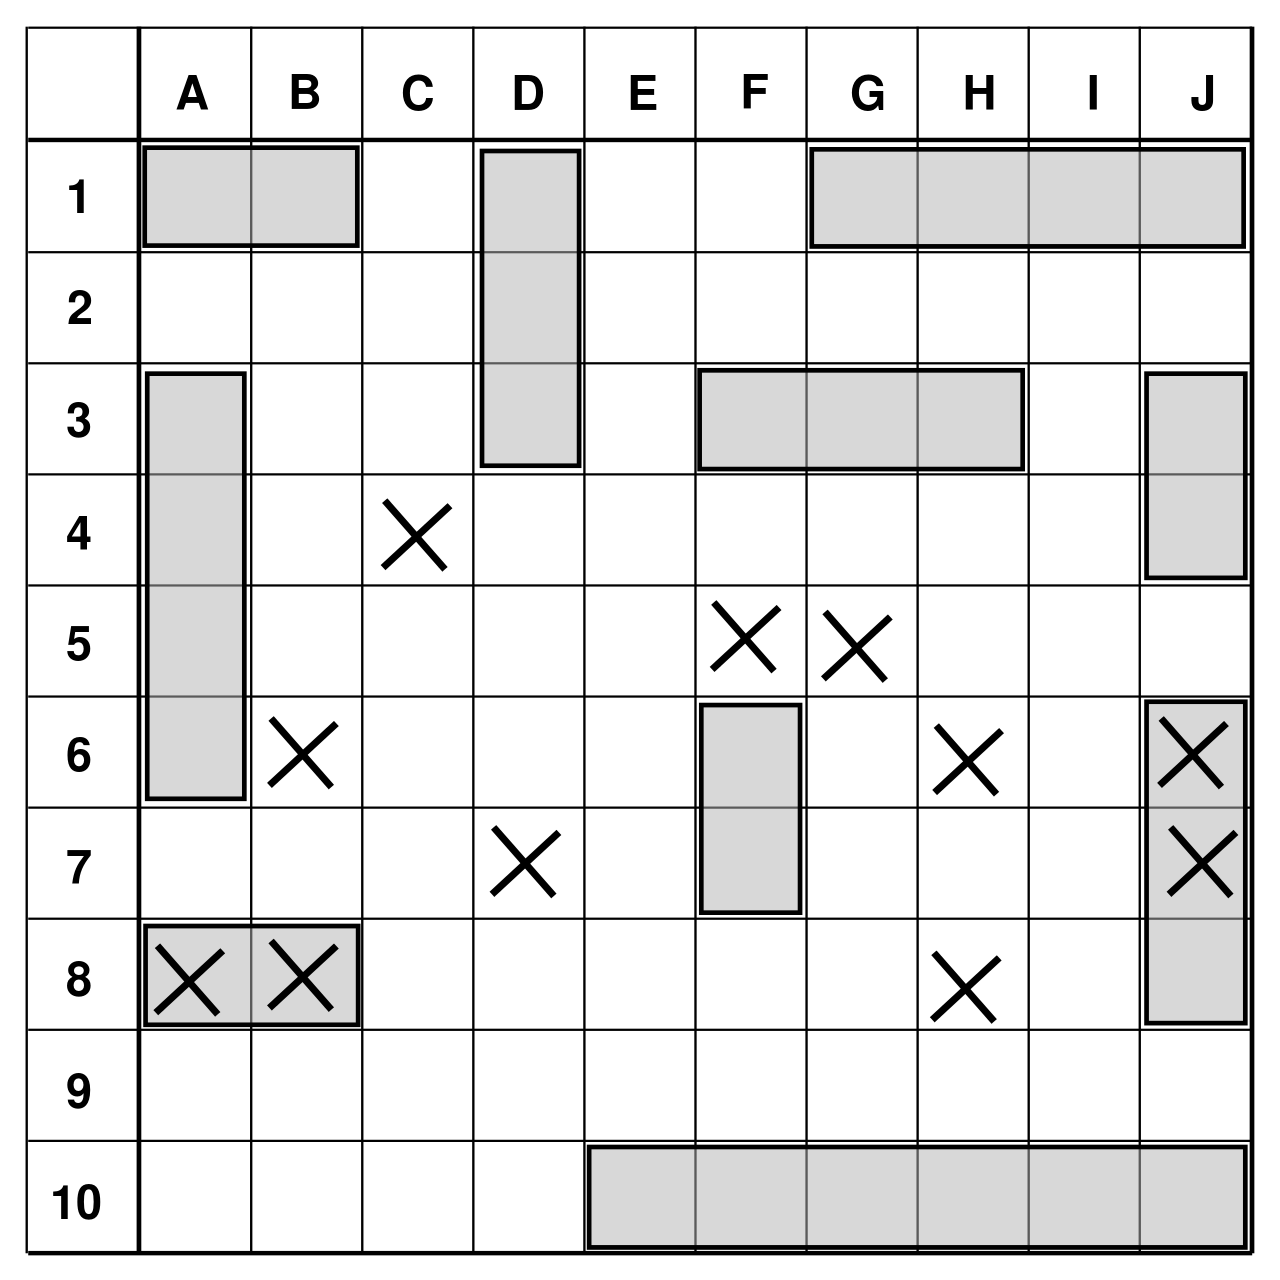
\includegraphics[scale=.25]{images/battleship}
  \caption[Battleship game board]{Ongoing battleship game on a 10 x 10 board. The grey boxes represent the battleships of varrying sizes, the white boxes water and the cross marks indicate either a hit, or a miss. Source: Reprinted from \cite{enwiki:1120935103}}
  \label{fig:battleship}
\end{figure}  